% Options for packages loaded elsewhere
\PassOptionsToPackage{unicode}{hyperref}
\PassOptionsToPackage{hyphens}{url}
\PassOptionsToPackage{dvipsnames,svgnames,x11names}{xcolor}
%
\documentclass[
  a4paper,
  DIV=11,
  numbers=noendperiod]{scrreprt}

\usepackage{amsmath,amssymb}
\usepackage{iftex}
\ifPDFTeX
  \usepackage[T1]{fontenc}
  \usepackage[utf8]{inputenc}
  \usepackage{textcomp} % provide euro and other symbols
\else % if luatex or xetex
  \usepackage{unicode-math}
  \defaultfontfeatures{Scale=MatchLowercase}
  \defaultfontfeatures[\rmfamily]{Ligatures=TeX,Scale=1}
\fi
\usepackage{lmodern}
\ifPDFTeX\else  
    % xetex/luatex font selection
\fi
% Use upquote if available, for straight quotes in verbatim environments
\IfFileExists{upquote.sty}{\usepackage{upquote}}{}
\IfFileExists{microtype.sty}{% use microtype if available
  \usepackage[]{microtype}
  \UseMicrotypeSet[protrusion]{basicmath} % disable protrusion for tt fonts
}{}
\makeatletter
\@ifundefined{KOMAClassName}{% if non-KOMA class
  \IfFileExists{parskip.sty}{%
    \usepackage{parskip}
  }{% else
    \setlength{\parindent}{0pt}
    \setlength{\parskip}{6pt plus 2pt minus 1pt}}
}{% if KOMA class
  \KOMAoptions{parskip=half}}
\makeatother
\usepackage{xcolor}
\setlength{\emergencystretch}{3em} % prevent overfull lines
\setcounter{secnumdepth}{-\maxdimen} % remove section numbering
% Make \paragraph and \subparagraph free-standing
\ifx\paragraph\undefined\else
  \let\oldparagraph\paragraph
  \renewcommand{\paragraph}[1]{\oldparagraph{#1}\mbox{}}
\fi
\ifx\subparagraph\undefined\else
  \let\oldsubparagraph\subparagraph
  \renewcommand{\subparagraph}[1]{\oldsubparagraph{#1}\mbox{}}
\fi


\providecommand{\tightlist}{%
  \setlength{\itemsep}{0pt}\setlength{\parskip}{0pt}}\usepackage{longtable,booktabs,array}
\usepackage{calc} % for calculating minipage widths
% Correct order of tables after \paragraph or \subparagraph
\usepackage{etoolbox}
\makeatletter
\patchcmd\longtable{\par}{\if@noskipsec\mbox{}\fi\par}{}{}
\makeatother
% Allow footnotes in longtable head/foot
\IfFileExists{footnotehyper.sty}{\usepackage{footnotehyper}}{\usepackage{footnote}}
\makesavenoteenv{longtable}
\usepackage{graphicx}
\makeatletter
\def\maxwidth{\ifdim\Gin@nat@width>\linewidth\linewidth\else\Gin@nat@width\fi}
\def\maxheight{\ifdim\Gin@nat@height>\textheight\textheight\else\Gin@nat@height\fi}
\makeatother
% Scale images if necessary, so that they will not overflow the page
% margins by default, and it is still possible to overwrite the defaults
% using explicit options in \includegraphics[width, height, ...]{}
\setkeys{Gin}{width=\maxwidth,height=\maxheight,keepaspectratio}
% Set default figure placement to htbp
\makeatletter
\def\fps@figure{htbp}
\makeatother
\newlength{\cslhangindent}
\setlength{\cslhangindent}{1.5em}
\newlength{\csllabelwidth}
\setlength{\csllabelwidth}{3em}
\newlength{\cslentryspacingunit} % times entry-spacing
\setlength{\cslentryspacingunit}{\parskip}
\newenvironment{CSLReferences}[2] % #1 hanging-ident, #2 entry spacing
 {% don't indent paragraphs
  \setlength{\parindent}{0pt}
  % turn on hanging indent if param 1 is 1
  \ifodd #1
  \let\oldpar\par
  \def\par{\hangindent=\cslhangindent\oldpar}
  \fi
  % set entry spacing
  \setlength{\parskip}{#2\cslentryspacingunit}
 }%
 {}
\usepackage{calc}
\newcommand{\CSLBlock}[1]{#1\hfill\break}
\newcommand{\CSLLeftMargin}[1]{\parbox[t]{\csllabelwidth}{#1}}
\newcommand{\CSLRightInline}[1]{\parbox[t]{\linewidth - \csllabelwidth}{#1}\break}
\newcommand{\CSLIndent}[1]{\hspace{\cslhangindent}#1}

\KOMAoption{captions}{tableheading}
\makeatletter
\makeatother
\makeatletter
\makeatother
\makeatletter
\@ifpackageloaded{caption}{}{\usepackage{caption}}
\AtBeginDocument{%
\ifdefined\contentsname
  \renewcommand*\contentsname{Table of contents}
\else
  \newcommand\contentsname{Table of contents}
\fi
\ifdefined\listfigurename
  \renewcommand*\listfigurename{List of Figures}
\else
  \newcommand\listfigurename{List of Figures}
\fi
\ifdefined\listtablename
  \renewcommand*\listtablename{List of Tables}
\else
  \newcommand\listtablename{List of Tables}
\fi
\ifdefined\figurename
  \renewcommand*\figurename{Figure}
\else
  \newcommand\figurename{Figure}
\fi
\ifdefined\tablename
  \renewcommand*\tablename{Table}
\else
  \newcommand\tablename{Table}
\fi
}
\@ifpackageloaded{float}{}{\usepackage{float}}
\floatstyle{ruled}
\@ifundefined{c@chapter}{\newfloat{codelisting}{h}{lop}}{\newfloat{codelisting}{h}{lop}[chapter]}
\floatname{codelisting}{Listing}
\newcommand*\listoflistings{\listof{codelisting}{List of Listings}}
\makeatother
\makeatletter
\@ifpackageloaded{caption}{}{\usepackage{caption}}
\@ifpackageloaded{subcaption}{}{\usepackage{subcaption}}
\makeatother
\makeatletter
\@ifpackageloaded{tcolorbox}{}{\usepackage[skins,breakable]{tcolorbox}}
\makeatother
\makeatletter
\@ifundefined{shadecolor}{\definecolor{shadecolor}{rgb}{.97, .97, .97}}
\makeatother
\makeatletter
\makeatother
\makeatletter
\makeatother
\ifLuaTeX
  \usepackage{selnolig}  % disable illegal ligatures
\fi
\IfFileExists{bookmark.sty}{\usepackage{bookmark}}{\usepackage{hyperref}}
\IfFileExists{xurl.sty}{\usepackage{xurl}}{} % add URL line breaks if available
\urlstyle{same} % disable monospaced font for URLs
\hypersetup{
  pdftitle={Macro Policy Brief: Global Inflation and the Oil Production Glut},
  pdfauthor={Krisna Gupta},
  colorlinks=true,
  linkcolor={blue},
  filecolor={Maroon},
  citecolor={Blue},
  urlcolor={Blue},
  pdfcreator={LaTeX via pandoc}}

\title{Macro Policy Brief: Global Inflation and the Oil Production Glut}
\author{Krisna Gupta}
\date{November 26, 2023}

\begin{document}
\maketitle
\begin{abstract}
Asumsi APBN menunjukkan optimisme pemerintah di mana dolar akan stabil
di 15000 Rp/US\$, inflasi di 2,8\% dan suku bunga di kisaran 6,7\%. Akan
tetapi, situasi global menunjukkan adanya kemungkinan suku bunga
internasional yang tetap tinggi untuk waktu yang lama (\emph{higher for
longer}). Di samping itu, kemungkinan adanya tekanan harga minyak
internasional akibat OPEC yang masih menahan produksi juga dapat
berdampak pada pasar minyak bumi di dalam negeri. Mengingat Indonesia
saat ini \emph{net importer}, maka akan sangat penting menjaga nilai
tukar dari ketidakpastian global.
\end{abstract}
\ifdefined\Shaded\renewenvironment{Shaded}{\begin{tcolorbox}[borderline west={3pt}{0pt}{shadecolor}, frame hidden, boxrule=0pt, breakable, interior hidden, sharp corners, enhanced]}{\end{tcolorbox}}\fi

\hypertarget{asumsi-apbn-2024}{%
\section{Asumsi APBN 2024}\label{asumsi-apbn-2024}}

Indonesia telah menentukan asumsi dasar APBN 2024 (Kementerian Keuangan
2023) seperti dapat dilihat pada Table~\ref{tbl-1}. Beberapa nilai di
asumsi ini nampak turun dibandingkan tahun sebelumnya di tahun 2023 dan
2022 (Santia 2022). Pemerintah sepertinya mengasumsikan bahwa inflasi
dan suku bunga tahun ini akan lebih rendah dibanding tahun-tahun
sebelumnya, dengan harga minyak dunia yang juga turun. Apakah ini asumsi
yang cukup tepat? Bagaimana implikasi dari deviasi asumsi-asumsi ini?

\hypertarget{tbl-1}{}
\begin{longtable}[]{@{}lll@{}}
\caption{\label{tbl-1}Asumsi makroekonomi APBN 2024}\tabularnewline
\toprule\noalign{}
Indikator & Nilai & Satuan \\
\midrule\noalign{}
\endfirsthead
\toprule\noalign{}
Indikator & Nilai & Satuan \\
\midrule\noalign{}
\endhead
\bottomrule\noalign{}
\endlastfoot
Pertumbuhan ekonomi & 5,2 & \% \\
Inflasi & 2,8 & \% \\
Nilai tukar rupiah & 15.000 & US\$ \\
Suku bunga SBN 10 tahun & 6,7 & \% \\
ICP & 82 & US\$/barel \\
\end{longtable}

\hypertarget{harga-minyak}{%
\section{Harga minyak}\label{harga-minyak}}

Harga minyak merupakan indikator yang paling relevan bagi Direktorat
Jenderal Minyak dan Gas (Ditjen Migas). Karena Indonesia merupakan net
importir minyak bumi, harga internasional menjadi semakin relevan, tidak
seperti batubara yang dapat direkayasa dengan kebijakan perdagangan
seperti \emph{Domestic Market Obligation} (DMO). Harga minyak dunia
(FRED 2023) dan produksi OPEC (ycharts.com 2023), organisasi penghasil
minyak terbesar, dapat dilihat di Figure~\ref{fig-oil}.

\begin{figure}

\begin{minipage}[t]{0.50\linewidth}

{\centering 

\raisebox{-\height}{

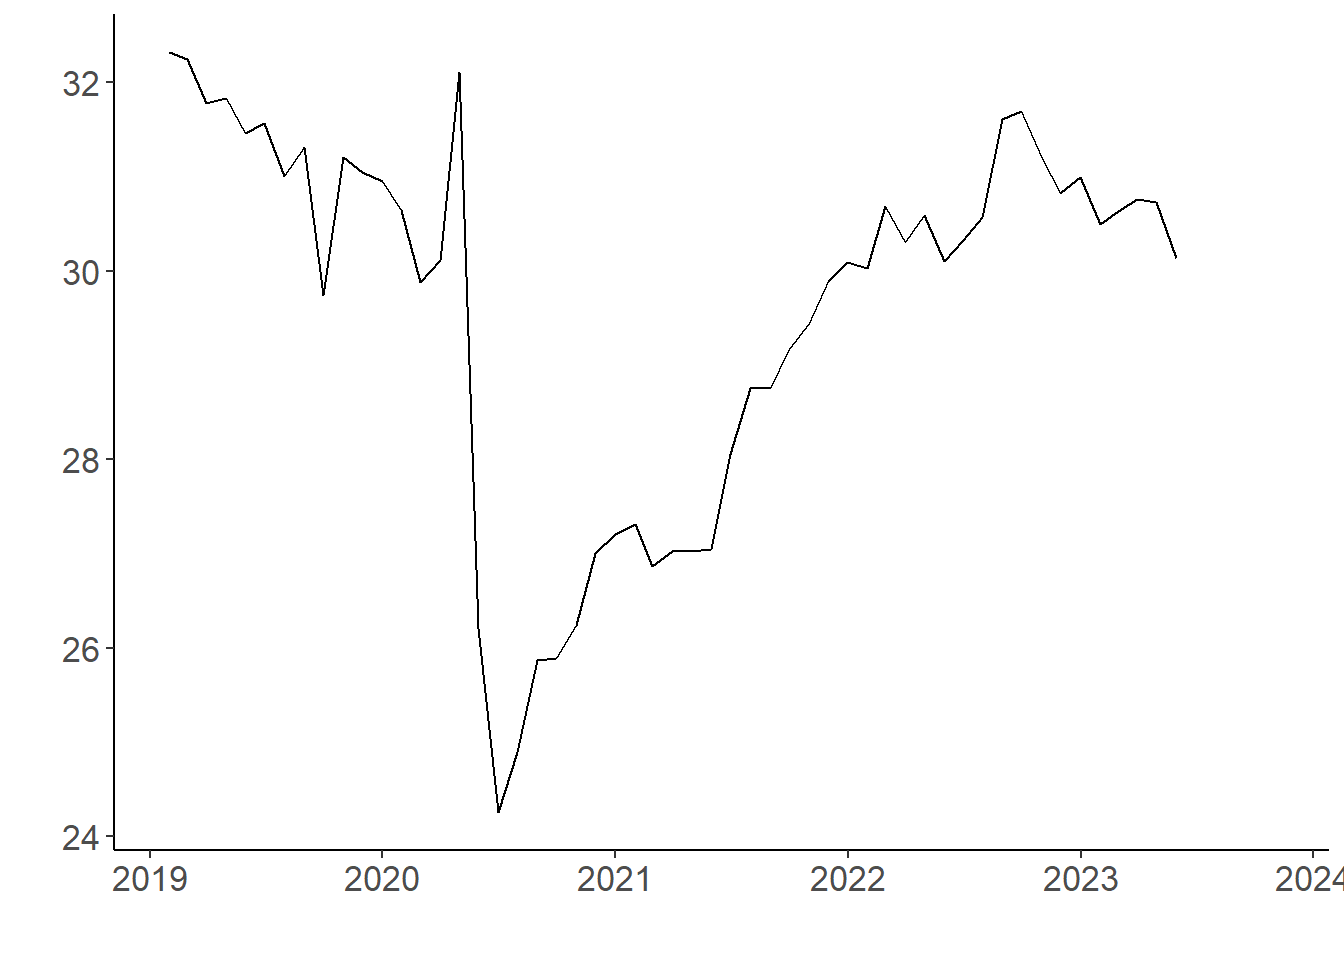
\includegraphics{index_files/figure-docx/fig-oil-1.png}

}

}

\subcaption{\label{fig-oil-1}Produksi crude oil OPEC (M/bbl/d)}
\end{minipage}%
%
\begin{minipage}[t]{0.50\linewidth}

{\centering 

\raisebox{-\height}{

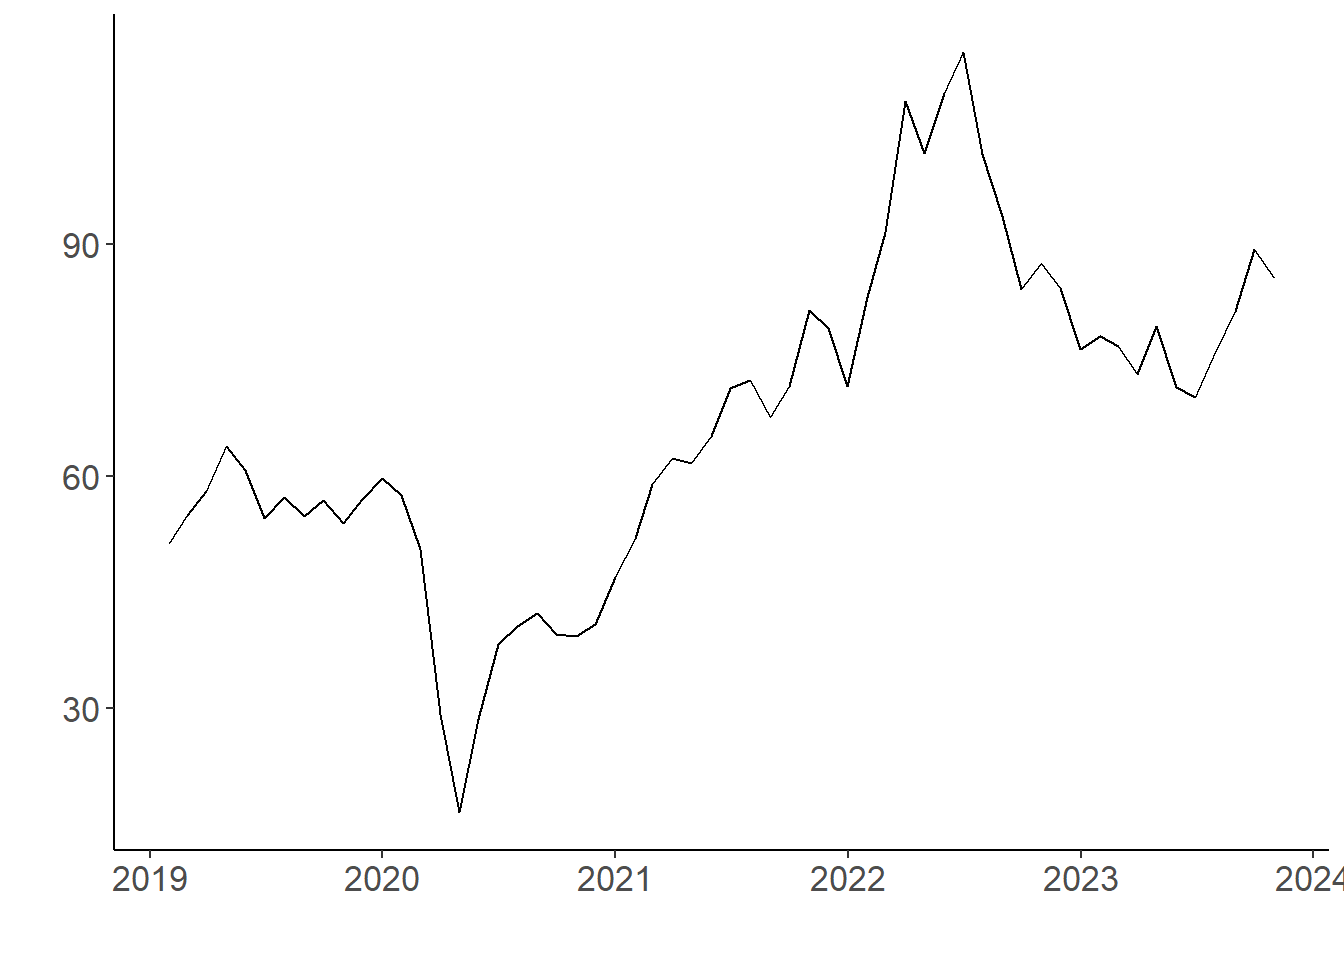
\includegraphics{index_files/figure-docx/fig-oil-2.png}

}

}

\subcaption{\label{fig-oil-2}Harga minyak WTI (USD/bbl)}
\end{minipage}%

\caption{\label{fig-oil}Kondisi minyak bumi di pasar global}

\end{figure}

Figure~\ref{fig-oil-1} menunjukkan adanya tren kenaikan produksi dari
negara-negara OPEC. Tren produksi minyak OPEC berkurang ketika COVID-19
masih merajalela, kemungkinan akibat lemahnya permintaan akibat
\emph{lockdown}. Peningkatan produksi perlahan terjadi dan menukik cukup
tajam tidak lama setelah perang Rusia-Ukraina terjadi. Peningkatan
produksi tersebut sudah mencapai tren 2019, namun tampak berhenti bahkan
cenderung menurun di pertengahan 2023.

Figure~\ref{fig-oil-2} menunjukkan tren harga yang serupa. Akan tetapi,
harga minyak WTI terus menanjak dan sudah tembus 110 USD/barrel pada
bulan Mei 2022. Namun, tren ini kembali menurun dan stagnan tak lama
kemudian. Akhir-akhir ini, harga minyak kembali naik ke level yang
sesuai dengan asumsi APBN. Meski demikian, OPEC masih berenacan untuk
menahan produksi untuk mengerek naik harga minyak (Seba 2023). Karena
itu pemerintah harus waspada.

\hypertarget{inflasi-global}{%
\section{Inflasi global}\label{inflasi-global}}

Inflasi global masih menjadi ancaman yang cukup pelik mengingat
terjadinya krisis baru di Timur Tengah. Bank Sentral Amerika Serikat
telah mengumumkan meski mereka mungkin akan menahan tingkat suku bunga
di level tinggi seperti saat ini namun untuk waktu yang panjang (Elena
2023). Hal ini membuat Indonesia harus waspada, karena jika tingkat suku
bunga masih akan tinggi, maka hal ini akan membuat Bank Indonesia (BI)
harus memilih antara mempertahankan rupiah dengan cara melepas devisa
atau dengan cara menaikkan suku bunga, atau bahkan membiarkan rupiah
melemah.

\begin{figure}

\begin{minipage}[t]{0.50\linewidth}

{\centering 

\raisebox{-\height}{

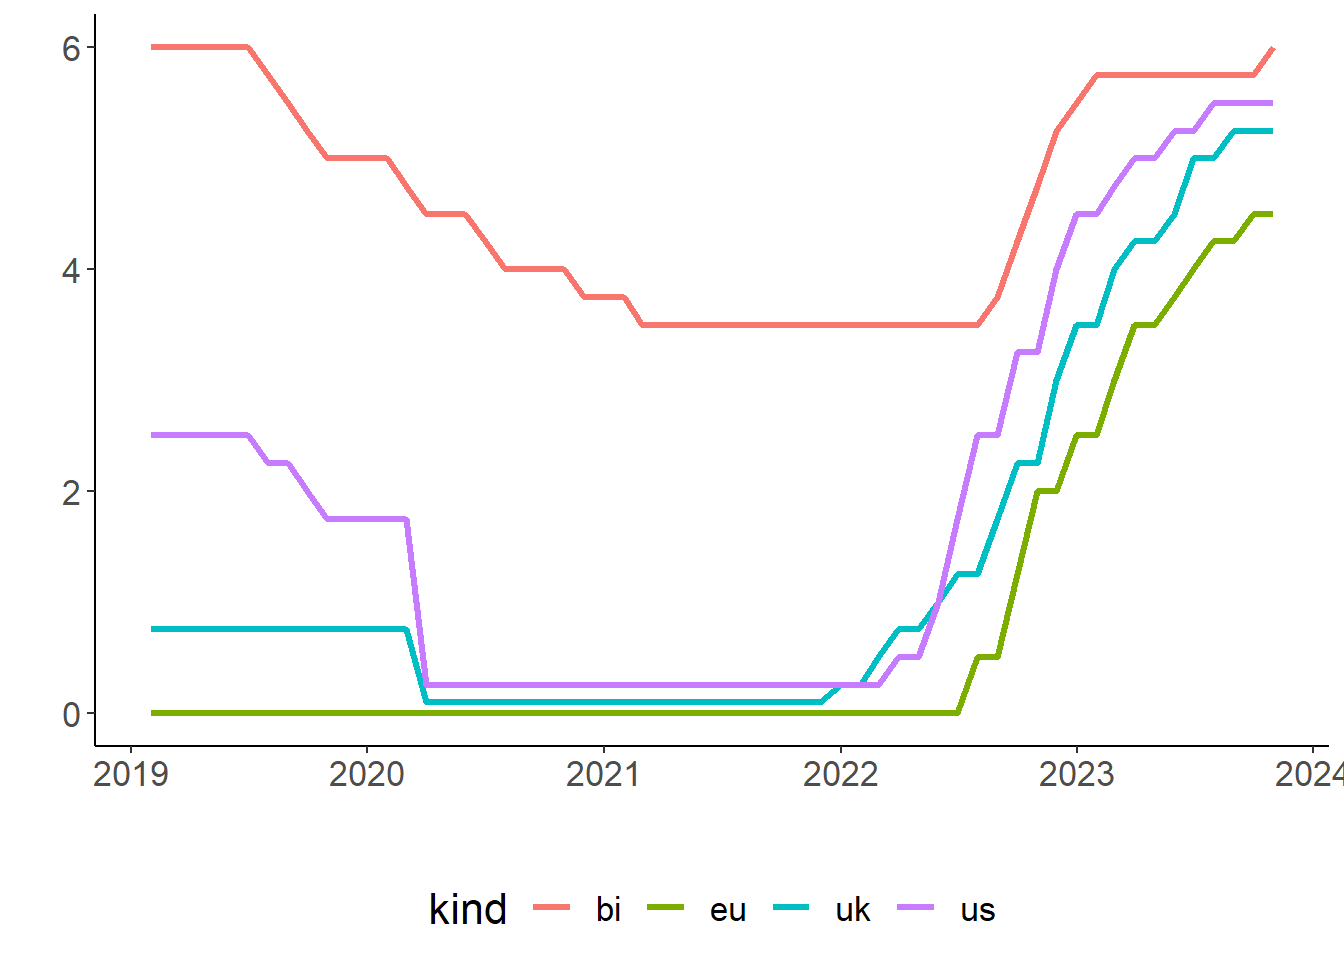
\includegraphics{index_files/figure-docx/fig-rate-1.png}

}

}

\subcaption{\label{fig-rate-1}Tingkat suku bunga beberapa negara (\%)}
\end{minipage}%
%
\begin{minipage}[t]{0.50\linewidth}

{\centering 

\raisebox{-\height}{

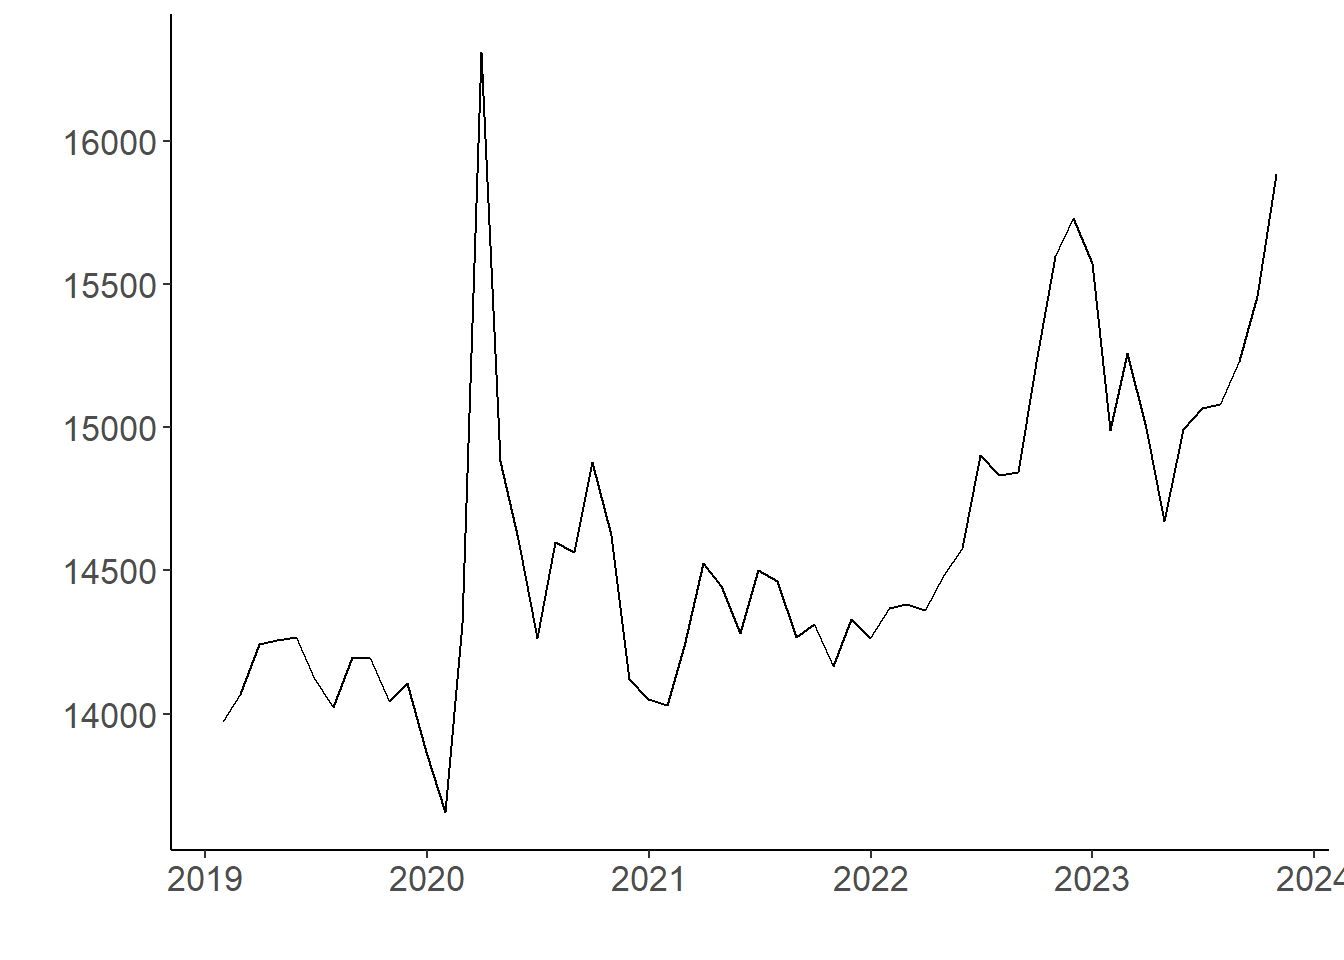
\includegraphics{index_files/figure-docx/fig-rate-2.png}

}

}

\subcaption{\label{fig-rate-2}Nilai tukar rupiah terhadap US\$
(Rp/US\$)}
\end{minipage}%

\caption{\label{fig-rate}Tingkat suku bunga dan mata uang rupiah}

\end{figure}

Sumber data pada Figure~\ref{fig-rate} adalah dari Bank Indonesia
(2023). Figure~\ref{fig-rate-1} menunjukkan tingginya \emph{policy rate}
dari negara-negara barat. Hal ini diakibatkan oleh tingginya inflasi di
jangka waktu tersebut sehingga bank sentral di negara-negara tersebut
harus menaikkan suku bunga. Bank Indonesia pun akhirnya harus mengikuti
demi mencegah larinya pemegang aset Rupiah ke negara-negara tersebut,
yang dapat mendorong pelemahan nilai tukar rupiah.

Dapat dilihat pada Figure~\ref{fig-rate-2} bahwa nilai tukar rupiah
cenderung melemah di sekitar jangka waktu yang sama seiring dengan
peningkatan suku bunga dari bank sentral negara barat. Meskipun rupiah
sempat kembali menguat di awal tahun 2023, namun berita ``higher for
longer'' kembali membuat investor menahan aset dolar lebih lama. BI pun
harus mengikuti kenaikan ini, seperti terlihat dari naiknya lagi suku
bunga BI baru-baru ini.

Di samping itu, ada potensi level rupiah akan \emph{floating} di posisi
yang lebih tinggi dibandingkan tren sebelumnya. Figure~\ref{fig-rate-1}
menunjukkan bahwa naiknya BI rate tidak setinggi negara-negara barat,
sehingga \emph{interest rate gap} Indonesia dengan negara-negara
tersebut mengecil. Jika BI tetap menjaga suku bunga di level ini, maka
ada kemungkinan rupiah akan tetap \emph{float} di posisi yang rendah dan
membuat asumsi makro bergeser.

\hypertarget{implikasi-ke-depan}{%
\section{Implikasi ke depan}\label{implikasi-ke-depan}}

Tren harga minyak dan inflasi global akan berpengaruh terhadap harga
minyak di Indonesia. Asumsi makro APBN 2024 bisa meleset akibat OPEC
yang berniat menjaga harga minyak agar tetap tinggi beserta dengan
kemungkinan tekanan terhadap nilai tukar rupiah. Tentunya hal ini juga
berpotensi menambah kenaikan biaya operasional Pertamina. Jika harga
dibiarkan floating, maka naiknya harga produk migas seperti BBM harus
diekspektasi. Tentunya hal ini tergantung apakah Bank Indonesia akan
bereaksi terhadap hal ini. Yang jelas, harus ada yang dikorbankan antara
tingkat suku bunga SBN dan nilai tukar rupiah jika tren ini terus
berlanjut.

\begin{figure}

\begin{minipage}[t]{0.50\linewidth}

{\centering 

\raisebox{-\height}{

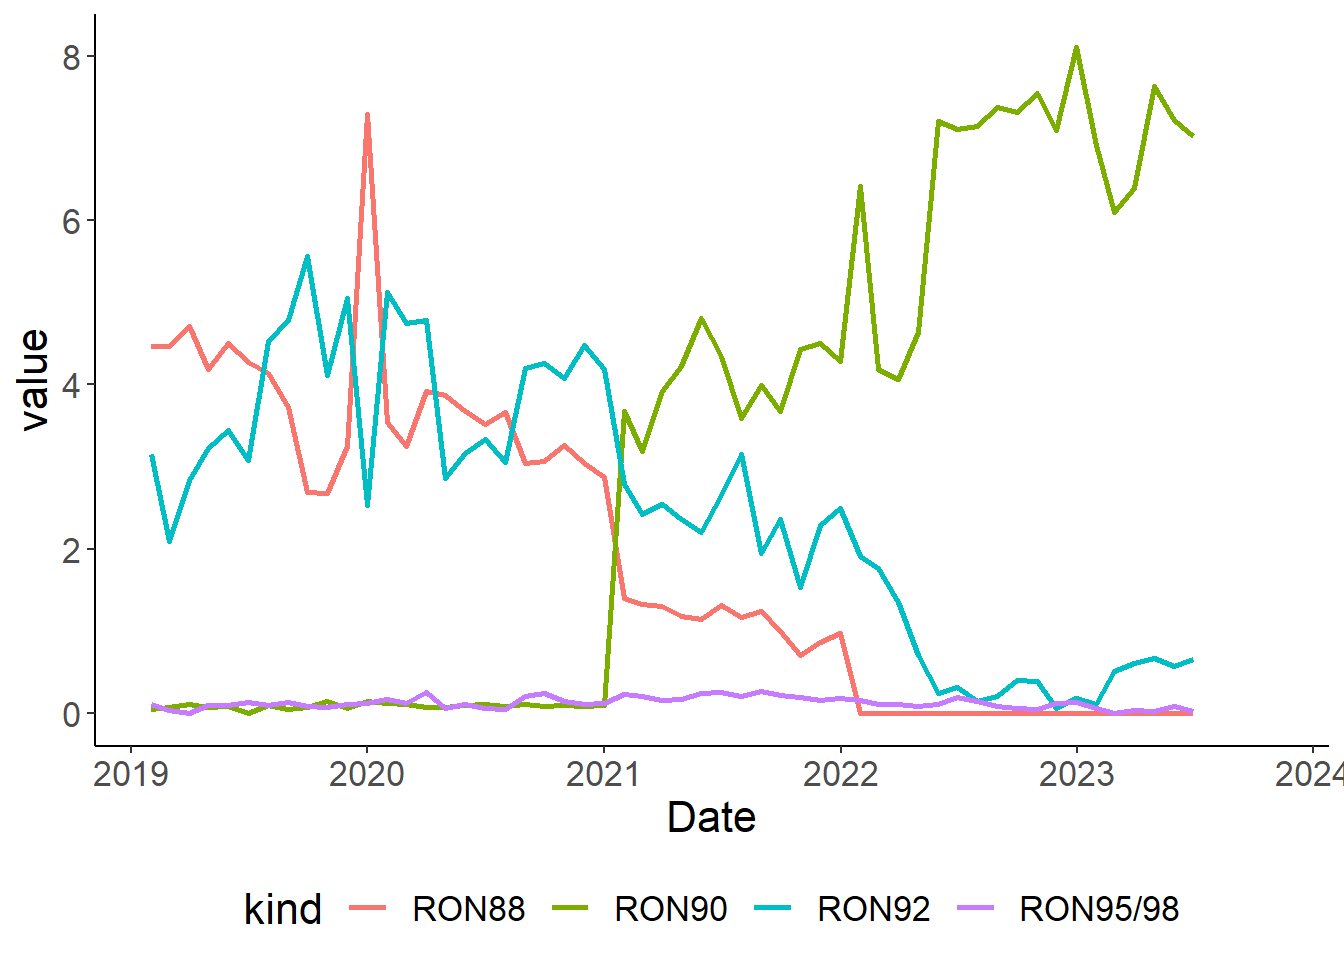
\includegraphics{index_files/figure-docx/fig-bbm-1.png}

}

}

\subcaption{\label{fig-bbm-1}Produksi BBM premium}
\end{minipage}%
%
\begin{minipage}[t]{0.50\linewidth}

{\centering 

\raisebox{-\height}{

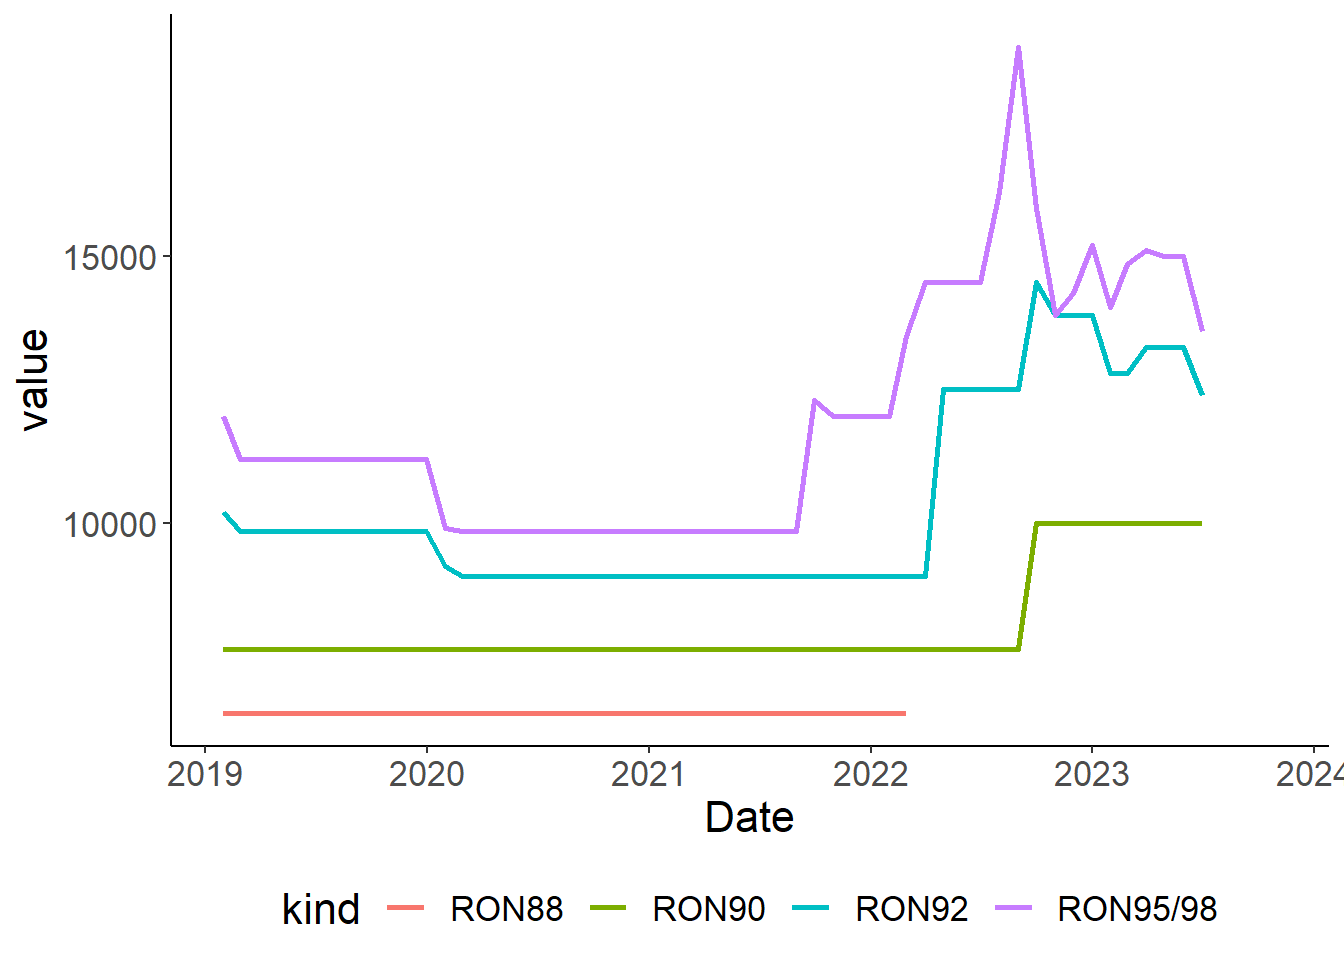
\includegraphics{index_files/figure-docx/fig-bbm-2.png}

}

}

\subcaption{\label{fig-bbm-2}Harga BBM premium (Rp/liter)}
\end{minipage}%

\caption{\label{fig-bbm}Kondisi harga dan konsumsi BBM di Indonesia}

\end{figure}

Melihat dampaknya langsung ke BBM mungkin cukup sulit. Hal ini karena
pasar BBM di Indonesia dikontrol dengan sangat ketat oleh pemerintah.
Dapat dilihat pada Figure~\ref{fig-bbm-1} bahwa konsumsi RON88 terjun
bebas karena produksi BBM jenis RON88 dihentikan. Sebelumnya,
diperkenalkan RON90 yang produksinya terus meningkat sampai sekarang.
Secara keseluruhan, produksi BBM masih tinggi.

Namun di sisi harga, tampak terlihat adanya kenaikan harga terutama
bensin RON tinggi yang naik lebih dulu seperti ditunjukkan oleh
Figure~\ref{fig-bbm-2}. Hal ini tentu imbas dari WTI juga naik di saat
yang hampir sama. Jika asumsi makro APBN meleset, maka hal ini
berpotensi menaikkan harga ke depannya.

Salah satu hal yang juga penting untuk dipertimbangkan adalah Program
Percepatan Kendaraan Bermotor Listrik Berbasis Baterai (KBLBB) telah
diamanatkan dalam Perpres Nomor 55 Tahun 2019 (Kementerian ESDM 2023).
Jika program ini berhasil, maka permintaan BBM bisa ditekan. Pasar
karbon juga bisa dimanfaatkan untuk menekan permintaan. Keseriusan
pemerintah dalam mencapai net zero di 2050 adalah satu aspek yang juga
perlu kita pertimbangkan (Gupta 2023).

\hypertarget{impulse-response-function}{%
\section{Impulse Response function}\label{impulse-response-function}}

Pada bagian ini dicoba ajukan sebuah usaha untuk mengestimasi dampak
dari gejolak global terhadap harga BMM RON tinggi. Metode yang digunakan
untuk studi awal ini adalah \emph{Vector Auto Regression} (VAR) untuk
melihat arah dari \emph{impulse response function} (IRF) dari perubahan
satu standar deviasi dari gejolak global (Pfaff 2007).

Pada percobaan kali ini digunakan 3 variabel, yaitu harga RON95/98
(\(p89\)), harga WTI (\(wti\)) dan nilai tukar rupiah terhadap dolar
(\(xr\)). Semua variabel dalam bulanan. RON95/98 dipilih karena harga
RON lain akan tergantung dari besarnya subsidi yang dialokasikan.
Dianggap bahwa RON paling tinggi adalah yang paling sensitif perubahan
harganya. WTI dan nilai tukar adalah proxy dari \emph{global production
glut} dan \emph{global inflation}. Series dapat dilihat di
Figure~\ref{fig-var}.

\begin{figure}

{\centering 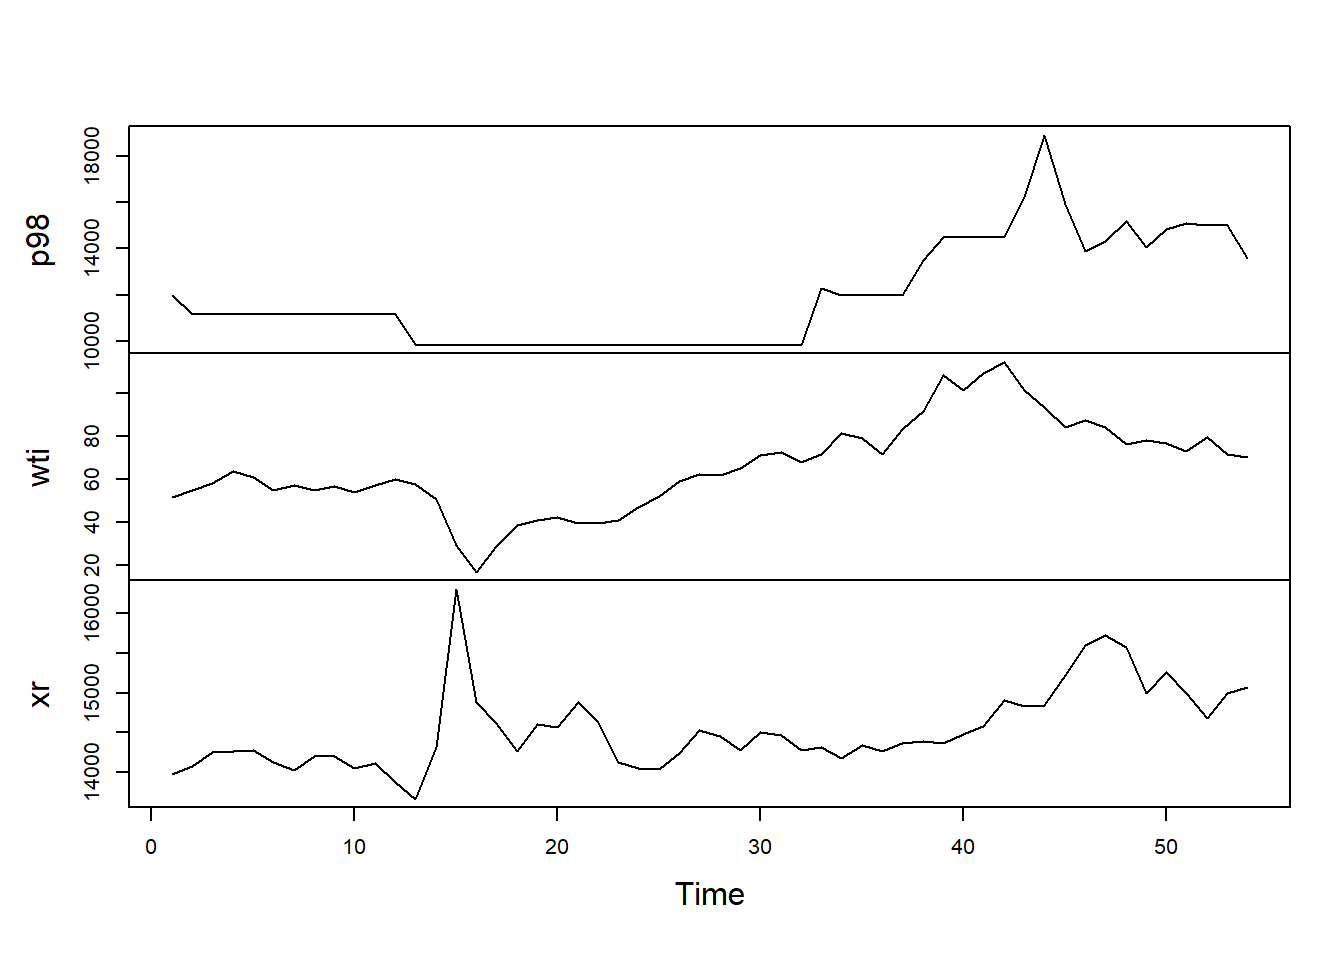
\includegraphics{index_files/figure-docx/fig-var-1.png}

}

\caption{\label{fig-var}Series 3 variabel}

\end{figure}

Model yang digunakan untuk studi awal ini adalah VAR(1). Dengan kata
lain, estimasi yang dilakukan adalah:

\[
\begin{aligned}
p98_t&=\beta_{10}+\beta_{11} p98_{t-1}+\beta_{12} wti_{t-1}+\beta_{13} xr_{t-1} \\
wti_t&=\beta_{20}+\beta_{21} p98_{t-1}+\beta_{22} wti_{t-1}+\beta_{23} xr_{t-1} \\
xr_t&=\beta_{30}+\beta_{31} p98_{t-1}+\beta_{32} wti_{t-1}+\beta_{33} xr_{t-1}
\end{aligned}
\]

Ekspektasi kita adalah bahwa harga dari RON95/98 dipengaruhi oleh harga
WTI dan nilai tukar, tapi tidak sebaliknya\footnote{\(X\) dikatakan
  \emph{granger cause} \(Y\) dan tidak sebaliknya jika \(X_{t-1}\)
  signifikan terhadap \(Y_t\) dan \(Y_{t-1}\) tidak signifikan terhadap
  \(X_t\)}. Artinya, kita harapkan signifikansi dari \(\beta_{12}\) dan
\(\beta_{13}\) namun kita harapkan \(\beta_{20}\) dan \(\beta_{30}\)
tidak signifikan. Di bawah ini adalah hasil dari VAR(1) tersebut:

\begin{verbatim}

VAR Estimation Results:
========================= 
Endogenous variables: p98, wti, xr 
Deterministic variables: const 
Sample size: 53 
Log Likelihood: -982.95 
Roots of the characteristic polynomial:
0.8842 0.8125 0.4743
Call:
VAR(y = wew, p = 1)


Estimation results for equation p98: 
==================================== 
p98 = p98.l1 + wti.l1 + xr.l1 + const 

         Estimate Std. Error t value Pr(>|t|)    
p98.l1  6.492e-01  8.322e-02   7.802 3.84e-10 ***
wti.l1  3.289e+01  7.991e+00   4.116 0.000147 ***
xr.l1   4.276e-01  2.413e-01   1.772 0.082658 .  
const  -4.159e+03  3.226e+03  -1.289 0.203342    
---
Signif. codes:  0 '***' 0.001 '**' 0.01 '*' 0.05 '.' 0.1 ' ' 1


Residual standard error: 761.8 on 49 degrees of freedom
Multiple R-Squared: 0.8941, Adjusted R-squared: 0.8877 
F-statistic:   138 on 3 and 49 DF,  p-value: < 2.2e-16 


Estimation results for equation wti: 
==================================== 
wti = p98.l1 + wti.l1 + xr.l1 + const 

         Estimate Std. Error t value Pr(>|t|)    
p98.l1  0.0003425  0.0007563   0.453   0.6527    
wti.l1  0.9296972  0.0726263  12.801   <2e-16 ***
xr.l1  -0.0038451  0.0021934  -1.753   0.0859 .  
const  56.7470688 29.3177376   1.936   0.0587 .  
---
Signif. codes:  0 '***' 0.001 '**' 0.01 '*' 0.05 '.' 0.1 ' ' 1


Residual standard error: 6.924 on 49 degrees of freedom
Multiple R-Squared: 0.901,  Adjusted R-squared: 0.895 
F-statistic: 148.7 on 3 and 49 DF,  p-value: < 2.2e-16 


Estimation results for equation xr: 
=================================== 
xr = p98.l1 + wti.l1 + xr.l1 + const 

        Estimate Std. Error t value Pr(>|t|)    
p98.l1 3.130e-02  4.063e-02   0.771  0.44469    
wti.l1 2.442e+00  3.901e+00   0.626  0.53429    
xr.l1  5.920e-01  1.178e-01   5.024 7.12e-06 ***
const  5.413e+03  1.575e+03   3.437  0.00121 ** 
---
Signif. codes:  0 '***' 0.001 '**' 0.01 '*' 0.05 '.' 0.1 ' ' 1


Residual standard error: 371.9 on 49 degrees of freedom
Multiple R-Squared: 0.4966, Adjusted R-squared: 0.4657 
F-statistic: 16.11 on 3 and 49 DF,  p-value: 2.03e-07 



Covariance matrix of residuals:
         p98     wti     xr
p98 580388.0  376.10 -19584
wti    376.1   47.94   -983
xr  -19583.8 -983.01 138337

Correlation matrix of residuals:
         p98     wti       xr
p98  1.00000  0.0713 -0.06911
wti  0.07130  1.0000 -0.38171
xr  -0.06911 -0.3817  1.00000
\end{verbatim}

Seperti kita lihat bahwa harga WTI sangat berpengaruh terhadap harga
RON95/98. Nilai tukar cukup berpengaruh meski signifikansinya ada di
level 8\%. Sementara itu, terbukti bahwa sebaliknya tidak terjadi:
\(p98_{t-1}\) tidak signifikan terhadap dua variabel lainnya.

berikutnya dilakukan impulse response function, yaitu apa yang terjadi
pada harga RON95/98 di jangka panjang jika ada \emph{shock} sebesar 1
standar deviasi terhadap harga WTI dan nilai tukar.

\begin{figure}

\begin{minipage}[t]{0.50\linewidth}

{\centering 

\raisebox{-\height}{

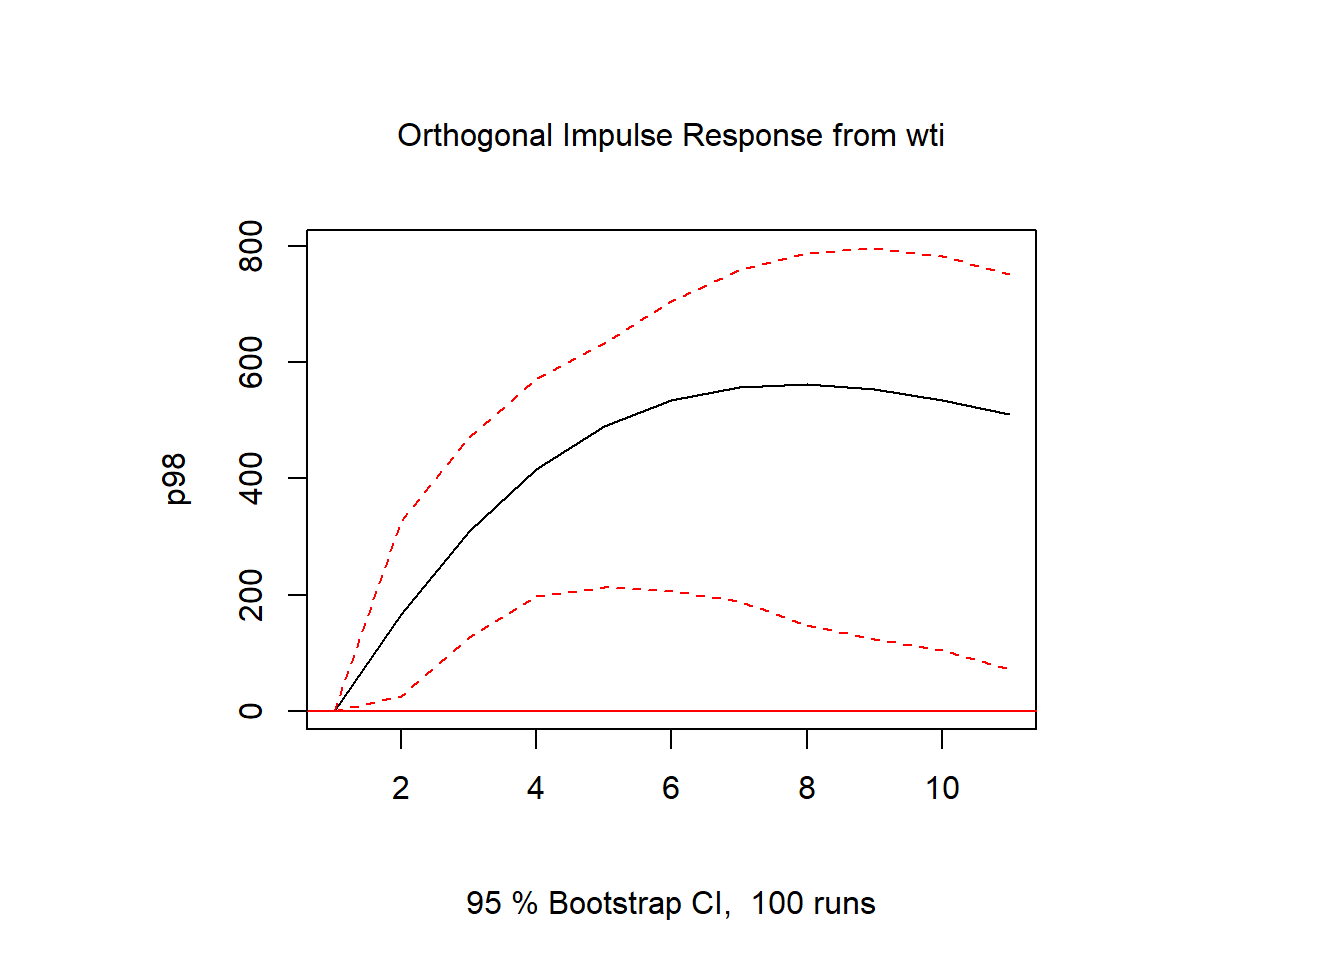
\includegraphics{index_files/figure-docx/fig-irf-1.png}

}

}

\subcaption{\label{fig-irf-1}IRF dari harga WTI}
\end{minipage}%
%
\begin{minipage}[t]{0.50\linewidth}

{\centering 

\raisebox{-\height}{

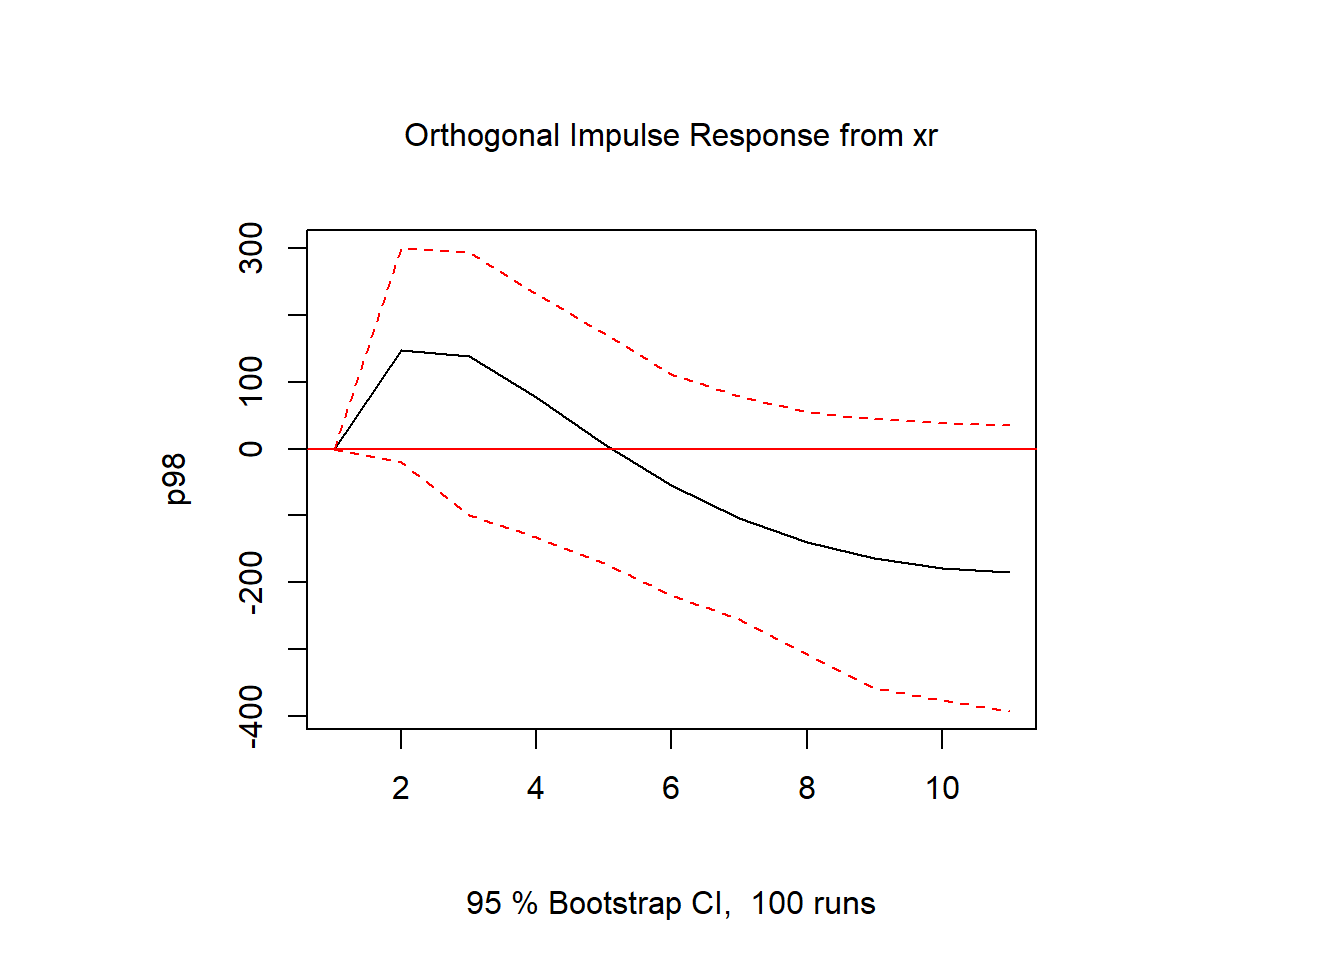
\includegraphics{index_files/figure-docx/fig-irf-2.png}

}

}

\subcaption{\label{fig-irf-2}IRF dari nilai tukar rupiah terhadap dolar
AS}
\end{minipage}%

\caption{\label{fig-irf}impulse response function dari VAR(1)}

\end{figure}

Dapat dilihat pada Figure~\ref{fig-irf-1} bahwa kenaikan harga WTI
sebanyak 1 standar deviasi mengakibatkan naiknya harga RON95/98 sampai
200 rupiah di bulan berikutnya. Kenaikan ini stabil di sekitar bulan
ke-7. Namun dapat dilihat bahwa standar deviasi dari estimasi ini cukup
lebar.

Dampak \emph{shock} dari nilai tukar sedikit berbeda (lihat
Figure~\ref{fig-irf-2}). Melemahnya nilai rupiah sebanyak 1 standar
deviasi mengakibatkan naiknya harga RON95/98, wajar mengingat BBM
sebagian besar harus diimpor. Namun dampak ini akan melemah dalam 3
bulan ke depan dan malah berkurang di jangka panjang. Mengingat bahwa
harga BBM dan nilai tukar di Indonesia seringkali diintervensi, maka
intervensi-intervensi tersebut juga masuk ke dalam estimasi.

Studi singkat ini cukup masuk akal, akan tetapi keandalan model ini
masih harus diperiksa. Berbagai metode lain juga dapat digunakan
tergantung dari asumsi, keandalan data, dan pertanyaan yang ingin
dijawab.

\hypertarget{refs}{}
\begin{CSLReferences}{1}{0}
\leavevmode\vadjust pre{\hypertarget{ref-seki}{}}%
Bank Indonesia. 2023. {``Statistik Ekonomi Dan Keuangan Indonesia.''}
Bank Indonesia.
\url{https://www.bi.go.id/id/statistik/ekonomi-keuangan/seki/Default.aspx\#headingThree}.

\leavevmode\vadjust pre{\hypertarget{ref-bisnis}{}}%
Elena, Maria. 2023. {``BI Peringatkan Fenomena Higher for Longer, Apa
Itu?''} bisnis.com.
\url{https://ekonomi.bisnis.com/read/20231023/9/1706962/bi-peringatkan-fenomena-higher-for-longer-apa-itu}.

\leavevmode\vadjust pre{\hypertarget{ref-fred}{}}%
FRED. 2023. {``FRED Economic Data.''}
\url{https://fred.stlouisfed.org/series/DCOILWTICO/}.

\leavevmode\vadjust pre{\hypertarget{ref-app}{}}%
Gupta, Krisna. 2023. {``Greening the Grid and What It Takes.''} Seminar
Nasional Politeknik APP Jakarta 2023.
\href{https://s.id/greenpln}{s.id/greenpln}.

\leavevmode\vadjust pre{\hypertarget{ref-esdm}{}}%
Kementerian ESDM. 2023. {``Pengembangan Ekosistem KBLBB Dorong Masuknya
Investasi Kendaraan Listrik.''} Siaran Pers Kementerian ESDM.
\url{https://ebtke.esdm.go.id/post/2023/09/14/3597/pengembangan.ekosistem.kblbb.dorong.masuknya.investasi.kendaraan.listrik\#:~:text=Program\%20Percepatan\%20Kendaraan\%20Bermotor\%20Listrik\%20Berbasis\%20Baterai\%20\%28KBLBB\%29,emisi\%20gas\%20rumah\%20kaca\%20serta\%20mencapai\%20tujuan\%20tersebut.}

\leavevmode\vadjust pre{\hypertarget{ref-apbn2024}{}}%
Kementerian Keuangan. 2023. {``APBN 2024 Resmi Meluncur.''} 2023.
\url{https://www.djkn.kemenkeu.go.id/berita/baca/33506/APBN-2024-Resmi-Meluncur.html}.

\leavevmode\vadjust pre{\hypertarget{ref-vars}{}}%
Pfaff, Bernhard. 2007. {``Using the Vars Package.''}
\url{https://www.researchgate.net/profile/David-Booth-7/post/How_to_select_optimal_lag_between_dependent_variable_and_independent_variables/attachment/59d649eb79197b80779a450a/AS\%3A473055043559424\%401489796519099/download/VARS_how_to_use.pdf}.

\leavevmode\vadjust pre{\hypertarget{ref-liputan6}{}}%
Santia, Tira. 2022. {``Tengok Perbandingan Asumsi Makro Dan Postur APBN
2022 Dan 2023.''} liputan6.com.
\url{https://www.liputan6.com/bisnis/read/5044185/tengok-perbandingan-asumsi-makro-dan-postur-apbn-2022-dan-2023?page=2}.

\leavevmode\vadjust pre{\hypertarget{ref-reuters}{}}%
Seba, Erwin. 2023. {``Oil Climbs over 2.''} Reuters.
\url{https://www.msn.com/en-us/money/markets/oil-climbs-over-2-as-opec-seen-deepening-cuts/ar-AA1kftku}.

\leavevmode\vadjust pre{\hypertarget{ref-yfin}{}}%
ycharts.com. 2023. {``OPEC Crude Oil Production.''}
\url{https://ycharts.com/indicators/opec_crude_oil_production}.

\end{CSLReferences}



\end{document}
